\documentclass[12pt]{article}
\usepackage[portuguese]{babel}
\usepackage[utf8]{inputenc}
\usepackage[T1]{fontenc}
\usepackage[pdftex]{graphicx}
\usepackage{float}
\usepackage{url}
\usepackage{lmodern}% http://ctan.org/pkg/lm

%\setlength{\parskip}{0.1cm}
\setlength{\paperheight}{29.7cm}
\setlength{\textheight}{23.0cm}
\setlength{\textwidth}{16.5cm}
\setlength{\oddsidemargin}{0.0cm}
\setlength{\topmargin}{-1.0cm}
%\pagestyle{empty}

\begin{document}

\begin{center}
{\sf {\large MAC-344 Arquitetura de Computadores}} \\
\vspace{0.5cm}
{\sf {\large Lista de Exercícios No. 2}}
\vspace{0.5cm}

\textbf{Lucas Sung Jun Hong (Nusp: 8124329)}
\end{center}

\paragraph{} Folha de respostas.

\begin{itemize}
  \item[{\bf 1.}] sd

  \item[{\bf 2.}] sd 

    \begin{figure}[ht]
      \caption{Observamos que a curva do processador avança mais em relação à memória.}
      \centering
        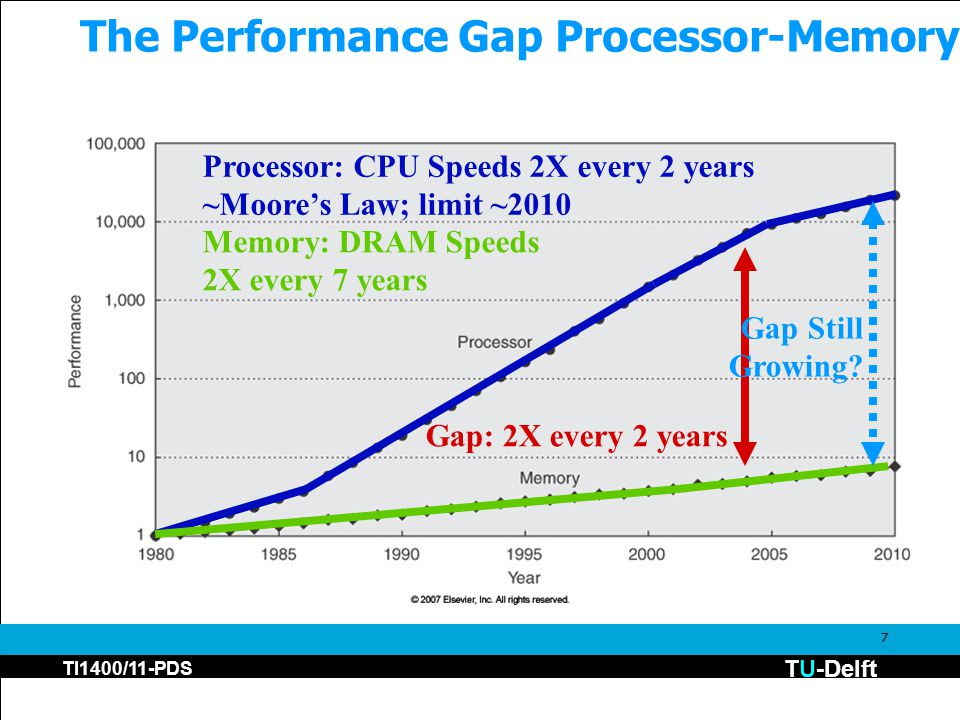
\includegraphics[width=0.8\textwidth]{img/slide_7.jpg}
    \end{figure}
    \vspace{0.5cm}

  \item[{\bf 3.}] sd 

  \item[{\bf 4.}] sd 

\end{itemize}

\end{document}
